\chapter{Introduction \\
\small{\textit{-- Author Name}}
\index{introduction} 
\index{Chapter!Introduction}
\label{Chapter::Introduction}}

 
All projects should have a small introduction.  Here we provide some
example LaTeX commands.  The first example, which is commented out in LaTeX,
is how to introduce an EPS file as an image into the document.

Here is a sample citation \cite{GM1998}.

\begin{verbatim}
\begin{figure}
\psfrag{a }{\Large stvDataObject}
\psfrag{b }{\large Object 1}
\psfrag{c }{\large Object 2}
\psfrag{d }{\large Object N}
\psfrag{e }{\large $Count:N$}
\psfrag{f }
{\hspace{-0.2in}\large \begin{tabular}{c} Sample \\ Table \end{tabular}}
\centering
\scalebox{1}{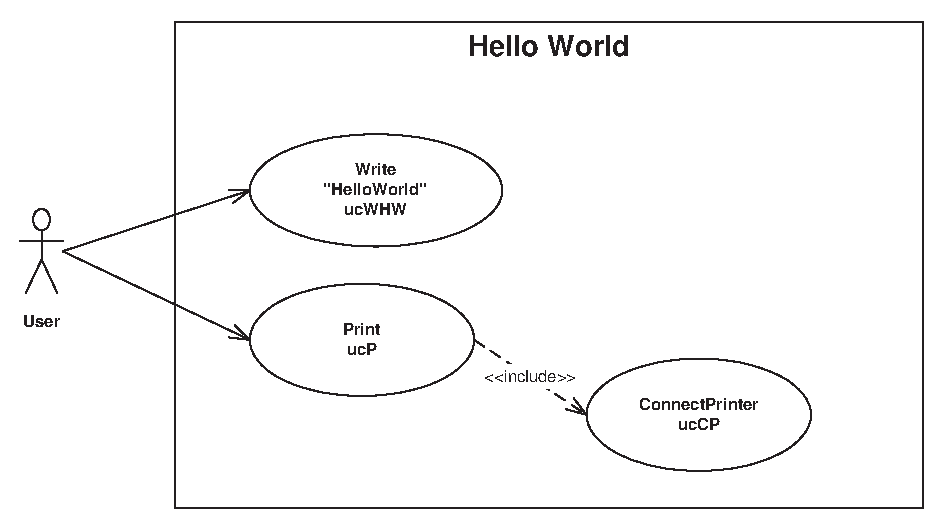
\includegraphics{eps/dsnHelloWorld.eps}}
\caption{\label{Figure::dsnHelloWolrd} Sample EPS image.}
\end{figure}
\end{verbatim}

\noindent
If using Overleaf, then you include a PNG or a JPG file as shown next:

\begin{verbatim}
\begin{figure}
\centering
\scalebox{0.8}{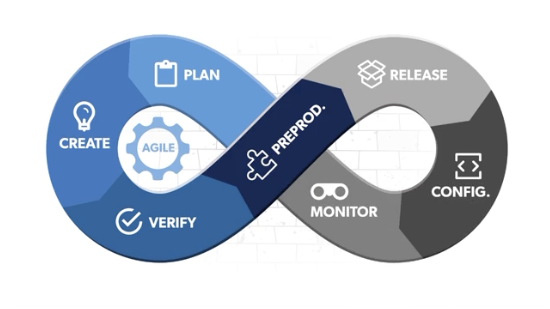
\includegraphics{png/stvAgileProcess.png}}
\caption{\label{Figure::stvAgile} PNG Image included.}
\end{figure}
\end{verbatim}

%\begin{figure}
%\centering
%\scalebox{0.8}{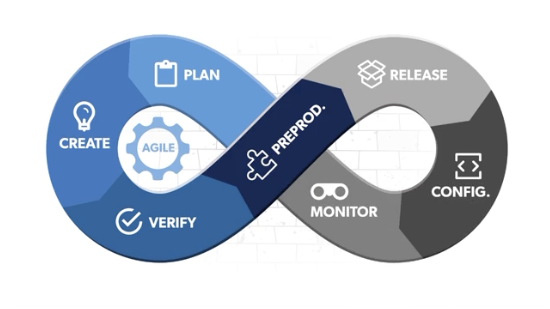
\includegraphics{png/stvAgileProcess.png}}
%\caption{\label{Figure::stvAgileProcess} PNG Image included.}
%\end{figure}

If compiling on Windows, as LaTeX-to-PDF (and not LaTeX-to-PS-to-PDF), 
you need to comment out the pdfmark package from itManual.tex:

\begin{verbatim}
%\usepackage[pdfmark, 
%breaklinks=true, 
%colorlinks=true,
%citecolor=blue,
%linkcolor=blue,
%menucolor=black,
%pagecolor=black,
%urlcolor=blue
%]{hyperref} % links in pdf
\end{verbatim}

\section{Compiling EPS files with PSFrag on Overleaf}

In the header file un-comment the following lines. (Viewable only in the .tex code, not in PDF):

	%\usepackage{graphicx} 
	%\usepackage[process=all]{pstool}
	%\usepackage[ 
	%breaklinks=true, 
	%colorlinks=true,
	%citecolor=blue,
	%linkcolor=blue,
	%menucolor=black,
	%urlcolor=blue
	%]{hyperref}
	%%%%%% 
	%%% NOTE IF LOADING hyperref PACKAGE
	%%% These lines are required ≥TL2020 due to 
	%%% incompatibility between hyperref and preview
	%%% (See https://github.com/latex3/hyperref/issues/166#issuecomment-760157370)
	%\makeatletter
	%\providecommand\HyPL@Entry[1]{}
	%\AddToHook{env/document/begin}{%
	%\@ifpackageloaded{preview}{
	%\ifPreview
		%\let\Hy@FirstPageHook\relax
		%\let\Hy@EveryPageAnchor\relax
	%\fi}{}}
	%\makeatother
	%\end{verbatim}
	%
	%\noindent
	%Then when using the image, use this syntax:
	%\begin{verbatim}
	%\begin{figure}
	%\centering
	%\psfragfig[width=1.0\linewidth]{<path to figure>}{
    %\psfrag{P0 }{\hspace{-0.5in} Test $\sum_0^N$ }
	%}
	%\caption{\label{<label name>} <Caption name>.}
	%\end{figure}

Note that with psfrag used this way, we cannot include references in the psfrag command.  
We can only replace text and use mathematical formulas.

Here is an example glossary term for \gls{should}.